
%\documentclass[icelandic]{beamer}

\documentclass[icelandic,a4paper,12pt]{article}
\usepackage{beamerarticle}

\mode<presentation>
{
  \usetheme{boxes}
  % með efnisyfirliti: Szeged, Frankfurt 
  % án efnisyfirlits: Pittsburgh
  % áhugavert: CambridgeUS, Boadilla
  %\setbeamercovered{transparent} %gegnsætt
  \setbeamercovered{invisible}
  }

\usepackage[english,icelandic]{babel}
\usepackage[utf8]{inputenc}
\usepackage{t1enc}
\selectlanguage{icelandic}
\usepackage{graphicx}
\usepackage{amsmath}
\usepackage{amssymb}
\usepackage{mathrsfs}
% \newcommand{\C}{{\mathbb  C}}
% \newcommand{\Z}{{\mathbb Z}}
% \newcommand{\R}{{\mathbb  R}}
% \newcommand{\N}{{\mathbb  N}}
% \newcommand{\Q}{{\mathbb Q}}
\renewcommand{\phi}{\varphi}
\renewcommand{\epsilon}{\varepsilon}

%\usepackage{pgfpages}
% \pgfpagesuselayout{2 on 1}[a4paper,border shrink=5mm]

\def\lecturename{Stærðfræðigreining IB}
\title{\insertlecture}
\author{Benedikt Steinar Magnússon, \href{mailto:bsm@hi.is}{bsm@hi.is}}
\institute
{
  Verkfræði- og náttúruvísindasvið\\
  Háskóli Íslands
}
\subtitle{Stærðfræðigreining IB}
%\subject{\lecturename}

\mode<article>
{
	\usepackage[colorlinks=false,
	pdfauthor={Benedikt Steinar Magnusson},
	pdftitle={IB: Namsefni
	}]{hyperref}
  %\usepackage{times}
  %\usepackage{mathptmx}
  \usepackage[left=1.5cm,right=4cm,top=1.5cm,bottom=3cm]{geometry}
}

% Beamer version theme settings

%\useoutertheme[height=0pt,width=2cm,right]{sidebar}
%\usecolortheme{rose,sidebartab}
%\useinnertheme{circles}
%\usefonttheme[only large]{structurebold}

\setbeamercolor{sidebar right}{bg=black!15}
\setbeamercolor{structure}{fg=blue}
\setbeamercolor{author}{parent=structure}

\setbeamerfont{title}{series=\normalfont,size=\LARGE}
\setbeamerfont{title in sidebar}{series=\bfseries}
\setbeamerfont{author in sidebar}{series=\bfseries}
\setbeamerfont*{item}{series=}
\setbeamerfont{frametitle}{size=}
\setbeamerfont{block title}{size=\small}
\setbeamerfont{subtitle}{size=\normalsize,series=\normalfont}

\defbeamertemplate*{footline}{infolines theme}
 {
   \leavevmode%
   \hbox{%
   \begin{beamercolorbox}[wd=.333333\paperwidth,ht=2.25ex,dp=1ex,center]{author in head/foot}%
   %  \usebeamerfont{author in head/foot}\insertshortauthor~~\beamer@ifempty{\insertshortinstitute}{}{(\insertshortinstitute)}
   \end{beamercolorbox}%
   \begin{beamercolorbox}[wd=.333333\paperwidth,ht=2.25ex,dp=1ex,center]{title in head/foot}%
    % \usebeamerfont{title in head/foot}\insertshorttitle
   \end{beamercolorbox}%
   \begin{beamercolorbox}[wd=.333333\paperwidth,ht=2.25ex,dp=1ex,right]{date in head/foot}%
     %\usebeamerfont{date in head/foot}\insertshortdate{}\hspace*{2em}
     \insertshortlecture.\insertframenumber{} / \insertshortlecture.\inserttotalframenumber\hspace*{2ex} 
   \end{beamercolorbox}}%
   \vskip0pt%
 }
  


\setbeamertemplate{sidebar right}
{
  {\usebeamerfont{title in sidebar}%
    \vskip1.5em%
    \hskip3pt%
    \usebeamercolor[fg]{title in sidebar}%
    \insertshorttitle[width=2cm-6pt,center,respectlinebreaks]\par%
    \vskip1.25em%
  }%
  {%
    \hskip3pt%
    \usebeamercolor[fg]{author in sidebar}%
    \usebeamerfont{author in sidebar}%
    \insertshortauthor[width=2cm-2pt,center,respectlinebreaks]\par%
    \vskip1.25em%
  }%
  \hbox to2cm{\hss\insertlogo\hss}
  \vskip1.25em%
  \insertverticalnavigation{2cm}%
  \vfill
  \hbox to 2cm{\hfill\usebeamerfont{subsection in
      sidebar}\strut\usebeamercolor[fg]{subsection in
      sidebar}\insertshortlecture.\insertframenumber\hskip5pt}%
  \vskip3pt%
}%

\setbeamertemplate{title page}
{
  \vbox{}
  \vskip1em
  %{\huge Kapitel \insertshortlecture\par}
  {\usebeamercolor[fg]{title}\usebeamerfont{title}\inserttitle\par}%
  \ifx\insertsubtitle\@empty%
  \else%
    \vskip0.25em%
    {\usebeamerfont{subtitle}\usebeamercolor[fg]{subtitle}\insertsubtitle\par}%
  \fi%     
  \vskip1em\par
  %Vorlesung \emph{\lecturename}\ vom 
  \insertdate\par
  \vskip0pt plus1filll
  \leftskip=0pt plus1fill\insertauthor\par
  \insertinstitute\vskip1em
}

%\logo{\includegraphics[width=2cm]{beamerexample-lecture-logo.pdf}}



% Article version layout settings

\mode<article>

\makeatletter
\def\@listI{\leftmargin\leftmargini
  \parsep 0pt
  \topsep 5\p@   \@plus3\p@ \@minus5\p@
  \itemsep0pt}
\let\@listi=\@listI


\setbeamertemplate{frametitle}{\paragraph*{\insertframetitle\
    \ \small\insertframesubtitle}\ \par
}
\setbeamertemplate{frame end}{%
  \marginpar{\scriptsize\hbox to 1cm{\sffamily%
      \hfill\strut\insertshortlecture.\insertframenumber}\hrule height .2pt}}
\setlength{\marginparwidth}{1cm}
\setlength{\marginparsep}{1.5cm}

\def\@maketitle{\makechapter}

\def\makechapter{
  \newpage
  \null
  \vskip 2em%
  {%
    \parindent=0pt
    \raggedright
    \sffamily
    \vskip8pt
    %{\fontsize{36pt}{36pt}\selectfont Kapitel \insertshortlecture \par\vskip2pt}
    {\fontsize{24pt}{28pt}\selectfont \color{blue!50!black} \insertlecture\par\vskip4pt}
    {\Large\selectfont \color{blue!50!black} \insertsubtitle, \@date\par}
    \vskip10pt

    \normalsize\selectfont \@author\par\vskip1.5em
    %\hfill BLABLA
  }
  \par
  \vskip 1.5em%
}

\let\origstartsection=\@startsection
\def\@startsection#1#2#3#4#5#6{%
  \origstartsection{#1}{#2}{#3}{#4}{#5}{#6\normalfont\sffamily\color{blue!50!black}\selectfont}}

\makeatother

\mode
<all>




% Typesetting Listings

\usepackage{listings}
\lstset{language=Java}

\alt<presentation>
{\lstset{%
  basicstyle=\footnotesize\ttfamily,
  commentstyle=\slshape\color{green!50!black},
  keywordstyle=\bfseries\color{blue!50!black},
  identifierstyle=\color{blue},
  stringstyle=\color{orange},
  escapechar=\#,
  emphstyle=\color{red}}
}
{
  \lstset{%
    basicstyle=\ttfamily,
    keywordstyle=\bfseries,
    commentstyle=\itshape,
    escapechar=\#,
    emphstyle=\bfseries\color{red}
  }
}



% Common theorem-like environments

\theoremstyle{definition}
\newtheorem{exercise}[theorem]{\translate{Exercise}}




% New useful definitions:

\newbox\mytempbox
\newdimen\mytempdimen

\newcommand\includegraphicscopyright[3][]{%
  \leavevmode\vbox{\vskip3pt\raggedright\setbox\mytempbox=\hbox{\includegraphics[#1]{#2}}%
    \mytempdimen=\wd\mytempbox\box\mytempbox\par\vskip1pt%
    \fontsize{3}{3.5}\selectfont{\color{black!25}{\vbox{\hsize=\mytempdimen#3}}}\vskip3pt%
}}

\newenvironment{colortabular}[1]{\medskip\rowcolors[]{1}{blue!20}{blue!10}\tabular{#1}\rowcolor{blue!40}}{\endtabular\medskip}

\def\equad{\leavevmode\hbox{}\quad}

\newenvironment{greencolortabular}[1]
{\medskip\rowcolors[]{1}{green!50!black!20}{green!50!black!10}%
  \tabular{#1}\rowcolor{green!50!black!40}}%
{\endtabular\medskip}



\lecture[1]{1. Föll og markgildi}{lecture-text}
\date{29. ágúst 2015}

\newcommand{\C}{{\mathbb  C}}
\newcommand{\Z}{{\mathbb Z}}
\newcommand{\R}{{\mathbb  R}}
\newcommand{\N}{{\mathbb  N}}
\newcommand{\Q}{{\mathbb Q}}
\begin{document}

\begin{frame}
	\maketitle
\end{frame}
\section*{Tölur og föll}
\subsection*{Inngangur}
\begin{frame}{Viðfangsefnið}
 \begin{block}{}
 \emph{There is a theory which states that if ever anybody discovers exactly what the Universe is for and 
  why it is here, it will instantly disappear and be replaced by something even more bizarre and inexplicable. 
  There is another theory which states that this has already happened.} \hfill -Douglas Adams
 \end{block}

\end{frame}

\begin{frame}{Stærðfræðigreining}

\begin{block}{Grunnhugmyndin}

 Stærðfræðigreining grundvallast á því að mæla breytingu (oft með tilliti til tíma)
 \begin{itemize}
  \item Eðlisfræði; hraði, hröðun, massi, orka, vinna, afl, þrýstingur
  \item Rúmmál; flatarmál, rúmmál, lengd, massamiðja
  \item Hagnýtingar; hagfræði, stofnstærðir, hámörkun/lágmörkun 
  \item Stærðfræði; markgildi, hermun, jafnvægisástand
 \end{itemize}
  \end{block}

\pause


\begin{block}{Sagan}
 Sett fram samtímis, en óháð, af Isaac Newton og Gottfried Leibniz í lok 17.~aldar.
\end{block}

%{\only{
\begin{figure}
 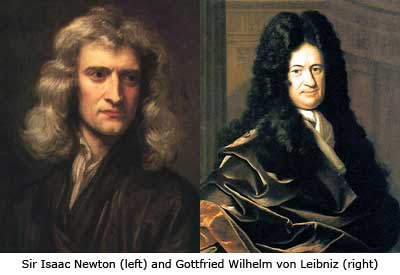
\includegraphics[width=4cm]{./myndir/kafli01/01_NewtonLeibniz.jpg}
 % NewtonLeibniz.jpg: 450x300 pixel, 72dpi, 15.88x10.58 cm, filebb=0 0 450 300
\end{figure}
%}<2>}



\end{frame}


\begin{frame}{Ítarefni}
 Fyrir nánari útlistun á hugtökunum sem við fjöllum um þá er hægt að skoða
\begin{itemize}
 \item \href{http://stae.is}{http://stæ.is} (hugtakasafn og orðaskrá)
  \item \href{http://planetmath.org}{http://planetmath.org}
  \item \href{http://mathworld.wolfram.com}{http://mathworld.wolfram.com}
  \item \href{http://en.wikipedia.org}{http://en.wikipedia.org} (ath.~enska útgáfan)
\end{itemize}

\pause
\begin{block}{Forrit}
 \begin{itemize}
  \item GeoGebra \href{http://www.geogebra.org}{http://www.geogebra.org}
  \item WolframAlpha \href{http://www.wolframalpha.com}{http://www.wolframalpha.com}
 \end{itemize}

\end{block}

\end{frame}


 \subsection{Skiladæmi}
 \subsubsection{Frágangur skiladæma}
 \begin{itemize}
 \item Skrifið upp {\bf dæmið} og lausnina snyrtilega
 \pause
 \item Vísið í setningar sem þið notið
 \pause
 \item Notið ekki rökfræðitákn eins og $\Leftarrow$, 
 $\Rightarrow$, $\Leftrightarrow$, $\wedge$, $\vee$
 \pause
 \item Textinn á að vera samfelldur og læsilegur (lesið hann 
 sjálf yfir)
 \pause
 \item Skýrt svar/niðurstaða
 \end{itemize}
 
 
\pause
\emph{"Forty-two!" yelled Loonquawl. "Is that all you've got to show 
for seven and a half million years' work?"}

\emph{"I checked it very thoroughly," said the computer, "and that 
quite definitely is the answer. I think the problem, to be quite 
honest with you, is that you've never actually known what the 
question is."} \hfill -Douglas Adams
 



\subsection*{Tölur}

\begin{frame}{Tölur}
\begin{block}{1.1 Skilgreining}
\begin{enumerate}[(i)]
\item  \emph{Náttúrlegu tölurnar} eru tölurnar
$1, 2, 3, 4, \ldots$ og mengi þeirra er táknað með $\N$.   \pause
\item Mengi \emph{heiltalna} er táknað með $\Z$. $\Z = \ldots,-2,-1,0,1,2,3,\ldots$\pause
\item Mengi \emph{ræðra talna} er táknað með $\Q$. $\Q = \{ \frac pq ; p,q \in \Z \}$.\pause
\item Mengi \emph{rauntalna} er táknað með $\R$.\pause
\item Mengi \emph{tvinntalna} er táknað með $\C$.
\end{enumerate}
\end{block}

\pause

\begin{block}{1.2 Athugasemd}  
Margir vilja telja $0$ með sem náttúrlega tölu.  Það er eðlilegt ef 
maður lítur á náttúrlegu tölurnar þannig að þær tákni fjölda.  Ef maður lítur hins vegar þannig
á að þær séu notaðar til að númera hluti
þá er 0 ekki með.
\end{block}

\end{frame}


\begin{frame}
\begin{block}{1.3 Smíði rauntalna}  Rauntölur eru smíðaðar úr ræðu tölunum
með því að fylla upp í götin. 

\pause

T.d.~eru 
\begin{eqnarray*}
\pi &=& 3,1415926\ldots, \qquad \text{og}\\
\sqrt 2 -4  &=& -2,58578\ldots
\end{eqnarray*}
ekki ræðar tölur (það er ekki hægt að skrifa þær sem brot $\frac ab$, 
þar sem $a$ og $b$ eru heilar tölur), en þær eru rauntölur.
\end{block}

\pause


\begin{block}{1.4 Frumsendan um efra mark}  
Látum $A$ vera mengi af  rauntölum
sem er þannig að til er tala $x$, þannig að 
fyrir allar tölur $a \in A$ þá er 
$$a\leq x.$$ 
Þá er til rauntala $x_0$ sem kallast {\em minnsta efra mark} fyrir
$A$, sem er þannig að  $a\leq x_0$ fyrir allar tölur $a\in
A$ og ef $x<x_0$ þá er til tala $a\in A$ þannig að $a>x$.  
\end{block}
\end{frame}


\begin{frame}{Bil}
\begin{block}{1.5 Skilgreining}  
Látum $a$ og $b$ vera rauntölur þannig að $a<b$.  
Skilgreinum 

(i) {\em opið bil}\ \ $(a,b)=\{x\in \R ; a<x<b\}$

(ii) {\em lokað bil}\ \ $[a,b]=\{x\in \R ; a\leq x\leq b\}$

(iii) {\em hálf opið bil}\ \ $[a,b)=\{x\in \R ; a\leq x<b\}$

(iv) {\em hálf opið bil}\ \ $(a,b]=\{x\in \R ; a< x\leq b\}$

\medskip

Þessi bil sem er skilgreind hér fyrir ofan eru kölluð endanleg.  Til
eru fleiri gerðir af bilum:


(v)  {\em opið óendanlegt bil}\ \    $(a,\infty)=\{x\in \R ; a<x\}$

(vi)  {\em opið óendanlegt bil}\ \    $(-\infty, a)=\{x\in \R ; x<a\}$

(vii)  {\em lokað óendanlegt bil} \ \ $[a,\infty)=\{x\in \R ; a\leq x\}$

(viii)  {\em lokað óendanlegt bil}\ \  $(-\infty, a]=\{x\in \R ; x\leq a\}$

(ix)  {\em allur rauntalnaásinn}\ \  $(-\infty, \infty)$.

\end{block}
\end{frame}

\begin{frame}
\begin{block}{1.6 Skilgreining} Mengi $A$ af rauntölum kallast bil ef um
allar tölur $a<b$ sem eru í menginu $A$ gildir að ef $a<x<b$ þá er $x$
líka í menginu $A$. \pause Þ.e.~\emph{engin göt}.
\end{block}

\pause

\begin{block}{1.7 Athugasemd}  

(i) Sérhvert bil á rauntalnaásnum er af
einni þeirra gerða sem talin er upp í Skilgreiningu 1.5.   (Þessi
staðhæfing er jafngild frumsendunni um efra mark.)

\pause

(ii) Það er jafngilt að segja 
$$x \in (a-\eta,a+\eta)$$ 
og 
$$|x-a| < \eta.$$
\end{block}
\end{frame}
\subsection*{Föll}	
\begin{frame}{Vörpun}
\begin{block}{1.8 Skilgreining}
\emph{Vörpun} frá mengi $X$ yfir í mengi $Y$ er regla sem úthlutar sérhverju
staki $x$ í $X$ nákvæmlega einu staki $f(x)$ í $Y$. Táknum þetta með
$f:X \to Y$. 

Stakið $f(x)$ kallast \emph{gildi} vörpunarinnar (í punktinum $x$).
\end{block}

\pause

\begin{block}
{1.9 Skilgreining}
Mengið $X$ kallast \emph{skilgreiningarmengi} $f$, 
mengið $Y$ kallast \emph{bakmengi} $f$ og 
mengið $f(X) = \{ f(x); x \in X \}$ kallast \emph{myndmengi} $f$.
\end{block}

\begin{center}
 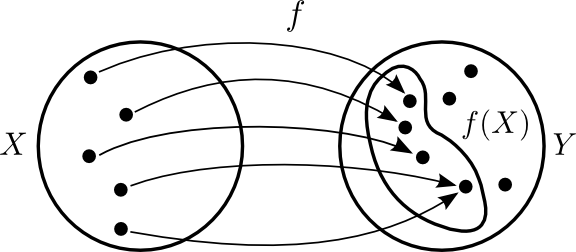
\includegraphics[width=7cm,keepaspectratio=true]{./myndir/kafli01/02_Mynd_vorpunar.png}
 % Mynd_vorpunar.eps: 277x122 pixel, 300dpi, 2.35x1.03 cm, bb=0 0 277 122
\end{center}
\end{frame}

\begin{frame}{Samskeyting}
\begin{block}{1.10 Skilgreining}
Látum $f:X \to Y$ og $g:Y \to Z$ vera varpanir. Vörpunin 
$g\circ f:X \to Z$ sem skilgreind er með 
$(g\circ f)(x)=g(f(x))$ kallast \emph{samskeyting} $f$ og 
$g$. 
Stakið 
$g(f(x)) \in Z$ fæst með því að beita fyrst vörpuninni $f$ á stakið 
$x$ og síðan vörpuninni $g$ á stakið $f(x)$.
\end{block}
% {\only{
% \begin{center}
%  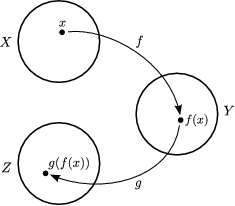
\includegraphics[width=4cm,keepaspectratio=true]{./myndir/kafli01/02_Samskeyting0.png}
%  % Mynd_vorpunar.eps: 277x122 pixel, 300dpi, 2.35x1.03 cm, bb=0 0 277 122
% \end{center}}<1>}
% \pause
% 
% {\only{
\begin{center}
 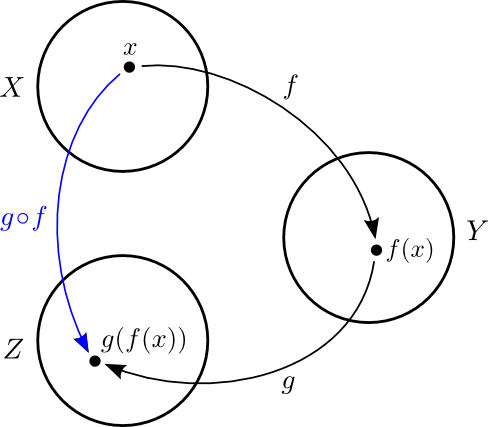
\includegraphics[width=4cm,keepaspectratio=true]{./myndir/kafli01/02_Samskeyting.png}
 % Mynd_vorpunar.eps: 277x122 pixel, 300dpi, 2.35x1.03 cm, bb=0 0 277 122
\end{center}
% }<2>}

\end{frame}

\begin{frame}{Eintækni/átækni}
\begin{block}{1.11 Athugasemd}
Það er ekki víst að öll gildin í $Y$ séu tekin (þ.e.~$f(X)$
getur verið minna en $Y$). Eins þá er mögulegt að $f$
taki sama gildið oftar en einu sinni.
\end{block}

\pause

\begin{block}{1.12 Skilgreining}
Við segjum að vörpunin $f$ sé \emph{átæk} ef $f(X)=Y$, það þýðir að 
fyrir sérhvert stak $y$ í $Y$ þá er til (amk.~eitt) stak
$x$ í $X$ þannig að $f(x)=y$.

\pause

Segjum að vörpunin $f$ sé \emph{eintæk} ef $f(x_1) = f(x_2)$ 
hefur í för með sér að $x_1=x_2$, þ.e.~sérhvert gildi sem
vörpunin tekur er bara tekið einu sinni.
\end{block}

\begin{center}
 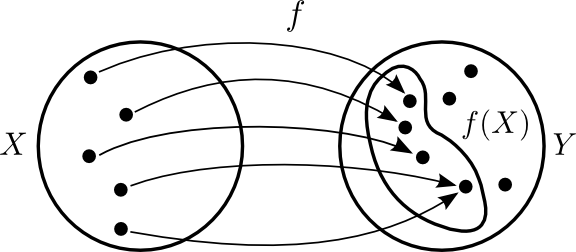
\includegraphics[width=6cm,keepaspectratio=true]{./myndir/kafli01/02_Mynd_vorpunar.png}
 % Mynd_vorpunar.eps: 277x122 pixel, 300dpi, 2.35x1.03 cm, bb=0 0 277 122
\end{center}

\end{frame}

\begin{frame}{Andhverfa}
 \begin{block}{1.13 Skilgreining}
  Vörpun sem er bæði eintæk og átæk kallast \emph{gagntæk}.
 \end{block}

 \pause
 
\begin{block}{1.14 Setning}
 Látum $f:X \to Y$ vera vörpun. Sagt er að 
$f$ sé andhverfanleg ef til er vörpun 
$f^{-1}:Y \to X$
þannig að samskeyting varpananna $f$ og 
$f^{-1}$ annars vegar og 
$f^{-1}$ og 
$f$ hins vegar sé viðeigandi 
samsemdarvörpun, þ.e.~$f^{-1}\circ f=id_X$ og
$f\circ f^{-1} = id_Y$.
\end{block}

% {\only{
% \begin{center}
%  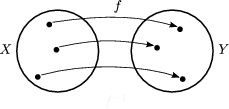
\includegraphics[width=7cm,keepaspectratio=true]{./myndir/kafli01/02_Andhverfa0.png}
%  % Mynd_vorpunar.eps: 277x122 pixel, 300dpi, 2.35x1.03 cm, bb=0 0 277 122
% \end{center}}<1>}
% 
% \pause
% 
% {\only{
\begin{center}
 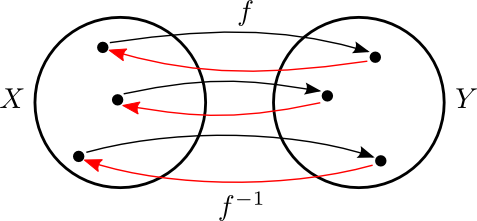
\includegraphics[width=7cm,keepaspectratio=true]{./myndir/kafli01/02_Andhverfa.png}
 % Mynd_vorpunar.eps: 277x122 pixel, 300dpi, 2.35x1.03 cm, bb=0 0 277 122
\end{center}
% }<2>}

\end{frame}

\begin{frame}{Graf}
\begin{block}{1.15 Athugasemd}
 Venjulega hjá okkur þá eru mengin $X$ og $Y$ mengi af rauntölum. Þegar $Y$ er
mengi af tölum þá er notast við orðið \emph{fall} í stað orðsins 
\emph{vörpun}.
\end{block}

\pause

\begin{block}{1.16 Skilgreining}
Látum $f:X \to Y$ vera fall þannig að $X$ og $Y$ eru mengi 
af rauntölum. \emph{Graf} fallsins $f$ er þá mengi allra punkta í planinu
$\R^2$ af gerðinni $(x,f(x))$ þar sem $x\in X$. 
Notum oft $y$ í stað $f(x)$.
\end{block}

\begin{center}
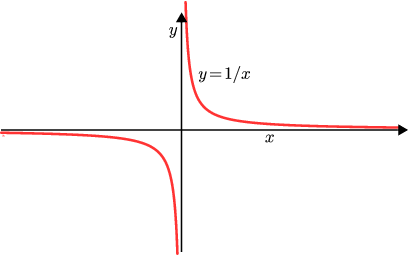
\includegraphics[width=7cm,keepaspectratio=true]{./myndir/kafli01/02_Graf.png}
 % Mynd_vorpunar.eps: 277x122 pixel, 300dpi, 2.35x1.03 cm, bb=0 0 277 122
\end{center}

\end{frame}

\end{document}
